%%%%%%%%%%%%%%%%%%%%%%%%%%%%%%%%%%%%%%%%%%%%%%%%%%%%%%%%%%%%%%%%%
% Dissertacao de Mestrado / Dept Fisica, CFM, UFSC              %
% Andre@UFSC - 2011                                             %
%%%%%%%%%%%%%%%%%%%%%%%%%%%%%%%%%%%%%%%%%%%%%%%%%%%%%%%%%%%%%%%%%


%:::::::::::::::::::::::::::::::::::::::::::::::::::::::::::::::%
%                                                               %
%                          Capítulo 4                           %
%                                                               %
%:::::::::::::::::::::::::::::::::::::::::::::::::::::::::::::::%

%***************************************************************%
%                                                               %
%                       Análise da Amostra                      %
%                                                               %
%***************************************************************%

% FIXME: Título do cap. 4
\chapter{Análise da amostra \STARLIGHTUV}
\label{sec:Analise}


%***************************************************************%
%                                                               %
%                  Análise - Diagrama cor -- cor                %
%                                                               %
%***************************************************************%

\section{Diagrama cor--cor}

De posse de uma amostra de galáxias com uma informação adicional (as magnitudes
em ultravioleta), é natural tentar ver como estas novas medidas se relacionam às
medidas conhecidas. \citet{Chilingarian2011} mostram que, num gráfico
tridimensional das cores $NUV-r$ e $g-r$ contra a magnitude $z$, a distribuição
de galáxias pode ser aproximada por uma superfície polinomial de baixa ordem. Os
autores mostram que há uma forte correlação entre a cor $NUV-r$ e a morfologia
da galáxia. Eles também estudam o histórico de formação estelar (SFH) no
diagrama $NUV-r$ contra $g-r$, mas a exploração é um tanto superficial.

Ainda segundo \citet[figura 1, exemplo na figura 4]{Chilingarian2011}, o
espalhamento dos dados na relação entre $g-r$ e $NUV-r$ é mais estreito na faixa
de magnitude $z$ entre $-24$ e $-20$. A densidade de galáxias da amostra
\starlight+UV em função de $g-r$ e $NUV-r$ (diagrama cor-cor) pode ser vista na
figura \ref{fig:DensityColor}. Apenas foram selecionados objetos com magnitude
$z$ entre $-23$ e $-21,5$. Este critério é utilizado em todos os diagramas de
cor contra cor presentes neste trabalho.

\begin{figure}
	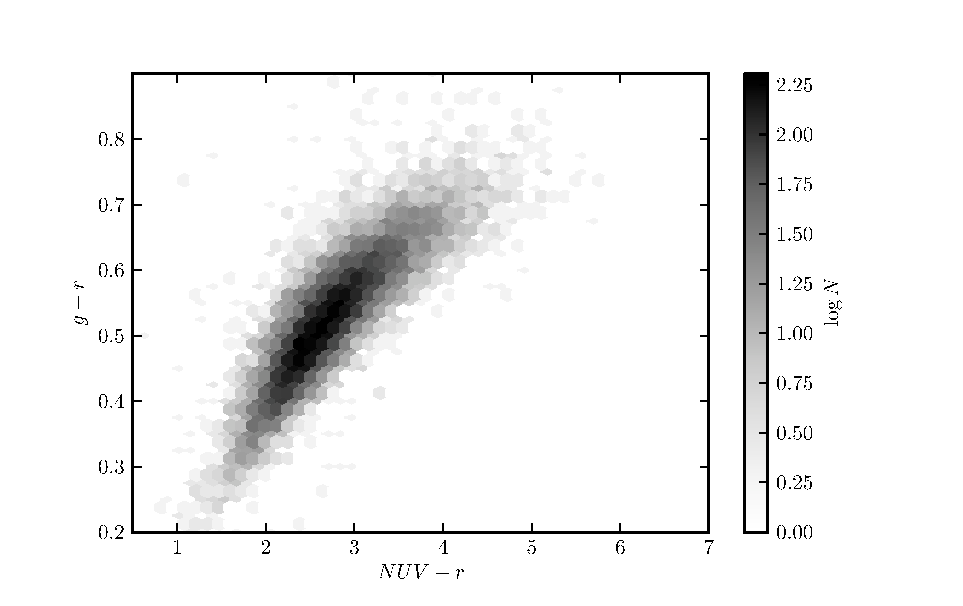
\includegraphics{figuras/uvcolor-color-density.eps}
	\caption[Densidade de galáxias no diagrama cor--cor UV.]
	{Densidade de galáxias em função de cor UV ($NUV-r$) e cor óptica ($g-r$). A
	intensidade dos bins hexagonais é o logaritmo do número de pontos dentro do
	bin, para melhorar a visualização. Esta figura é similar à figura 4 de
	\citet{Chilingarian2011}. Foram selecionados objetos da amostra do \starlight
	com magnitude na banda $z$ entre $-23$ e $-21,5$ e {\em redshift} entre $0,04$
	e $0,17$. As magnitudes $g$, $r$ e $z$ são do \SDSS.}
	\label{fig:DensityColor}
\end{figure}

A figura \ref{fig:ColorStarlightParam} mostra os parâmetros físicos das galáxias
obtidos através do \starlight no diagrama cor--cor. Essencialmente, os gráficos
são os mesmos que o da figura \ref{fig:DensityColor}, com a cor dos pontos
indicando o valor de cada parâmetro. Em especial, o painel (a) mostra a relação
entre a idade média (ponderada em fluxo das SSP) e a cor das galáxias.
\citeauthor{Chilingarian2011} chegam numa relação semelhante, porém por outros
meios.

\begin{figure}
	\includegraphics{figuras/uvcolor-color.eps}
	\caption[Diagrama cor--cor UV para os diversos parâmetros \starlight.]
	{Parâmetros físicos das galáxias em função de cor UV e cor óptica. O contorno
	das figuras representam os níveis referentes à figura \ref{fig:DensityColor},
	e os eixos horizontal e vertical são os mesmos. As cores dos pontos nos painéis
	correspondem a: \textbf{(a)} Logaritmo da idade média da galáxia, ponderada
	pelo fluxo das SSP componentes. \textbf{(b)} O mesmo que a anterior, mas
	ponderada pela massa das SSP. \textbf{(c)} Metalicidade média da galáxia
	ponderada pelo fluxo das SSP cmponentes. \textbf{(d)} O mesmo que a
	anterior, ponderada pela massa das SSP. \textbf{(e)} Logaritmo da massa
	estelar da galáxia, em massas solares. \textbf{(f)} Extinção por poeira na
	galáxia, na banda $V$.}
	\label{fig:ColorStarlightParam}
\end{figure}


%***************************************************************%
%                                                               %
%                     Análise - Classificação                   %
%                                                               %
%***************************************************************%

\section{Classificação das galáxias}

Nesta seção são discutidas formas de classificação de galáxias, e a forma como a
cor UV das galáxias está relacionada às classes. São utilizadas as linhas de
emissão \Halpha, \Hbeta, \NII e \OIII (daqui em diante chamados apenas de \nII e
\oIII).

O diagrama WHAN relaciona a largura equivalente da linha \Halpha ($\WHa$) com a
razão entre o fluxo das linhas \nII e \Halpha ($\nII/\Halpha$). As galáxias são
separadas em classes conforme os critérios a seguir \citep{CidFernandes2011}.

% FIXME: Usar lista para critérios do WHAN
\begin{list}{}{\setlength\itemsep{0pt}}
\item \textbf{(a)} Galáxias com formação estelar (SFG): $\log{\nII/\Halpha} <
-0,4$ e $\WHa > 3\text{\AA}$,
\item \textbf{(b)} Galáxias com núcleo ativo forte (sAGN): $\log{\nII/\Halpha} >
-0,4$ e $\WHa > 6\text{\AA}$,
\item \textbf{(c)} Galáxias com núcleo ativo fraco (wAGN): $\log{\nII/\Halpha} >
-0,4$ e $3\text{\AA} > \WHa > 6\text{\AA}$,
\item \textbf{(d)} Galáxias ``aposentadas'' (RG): $\WHa < 3\text{\AA}$,
\item \textbf{(e)} Galáxias passivas (PG): $\WHa < 0,5\text{\AA}$ e $\WnII <
0,5\text{\AA}$.
\end{list}

O diagrama WHAN para a amostra \starlightUV pode ser visto na figura
\ref{fig:Whan}. A cor dos pontos para cada classe é o mesmo utilizado por
\citet{CidFernandes2011}. São $59\,180$ galáxias com formação estelar, $39\,053$
galáxias com núcleo ativo forte, $14\,647$ galáxias com núcleo ativo fraco,
$29\,119$ galáxias aposentadas e $19\,939$ galáxias passivas. O mesmo diagrama,
agora com a cor dos pontos representando a cor $NUV-r$ das galáxias (figura
\ref{fig:WhanUV}), mostra que a cor das galáxias está relacionada à sua classe.

\begin{figure}
	\includegraphics{figuras/whan.eps}
	\caption[Diagrama de diagnóstico WHAN.]
	{Diagrama de diagnóstico WHAN. As linhas tracejadas separam as galáxias
	em classes. \textbf{Azul}: galáxias com formação estelar (SFG). \textbf{Verde
	claro}: galáxias com núcleo ativo forte (sAGN). \textbf{Verde forte}:
	galáxias com núcleo ativo fraco (wAGN). \textbf{Preto}: galáxias aposentadas
	(RG). \textbf{Vermelho}: galáxias passivas (PG). \textbf{Magenta}: Galáxias
	que não se encaixam em nenhuma destas classes.}
	\label{fig:Whan}
\end{figure}

\begin{figure}
	\includegraphics{figuras/whan-uv.eps}
	\caption[Cores ultravioleta no diagrama WHAN.]
	{Diagrama WHAN semelhante ao da figura \ref{fig:Whan}. A cor dos pontos
	representa $NUV-r$. Pode-se notar que a cor típica dos pontos muda para cada
	classe.}
	\label{fig:WhanUV}
\end{figure}

Outra forma de classificar as galáxias é através das razões entre linhas de
emissão $\nII/\Halpha$ e $\oIII/\Hbeta$. Este diagrama de diagnóstico é
conhecido como BPT. Em \citet{CidFernandes2010} discute-se os detalhes desta
forma de classificação utilizando o diagrama BPT. As linhas tracejadas separam
as galáxias nas classes {\em Seyfert} (correspondendo às sAGN no diagrama WHAN),
{\em LINER} (wAGN e aposentadas no WHAN) e galáxias de formação estelar (SFG). A
cor UV das galáxias da amostra no diagrama BPT (figura \ref{fig:BPTUV}) é
consistente com as cores para o diagrama WHAN.

\begin{figure}
	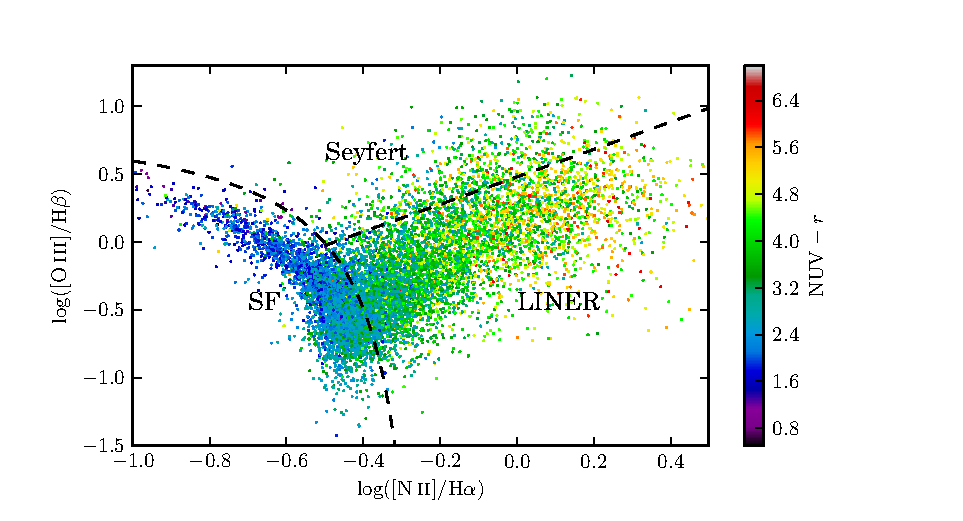
\includegraphics{figuras/bpt-uv.eps}
	\caption[Cores ultravioleta no diagrama BPT.]
	{Diagrama BPT, também usado para classificar galáxias. A cor dos
	pontos representa $NUV-r$. As linhas tracejadas separam das galáxias nas
	classes {\em Seyfert}, {\em LINER} e formação estelar, conforme
	\citet[linhas S06 e K06 da tabela 1]{CidFernandes2010}.}
	\label{fig:BPTUV}
\end{figure}

As classes de galáxias ocupam regiões diferentes do diagrama cor--cor. Na figura
\ref{fig:ColorClass} a cor dos pontos representa a classe das galáxias da mesma
forma que na figura \ref{fig:Whan}. Embora não esteja muito claro para as
classes RG e PG, as classes formam uma sequência no diagrama cor--cor. Isto pode
ser visto mais facilmente na figura \ref{fig:HistogramaCorClasse}. Esta figura é
de certo modo uma versão resumida da figura \ref{fig:ColorClass}. Embora haja
uma sobreposição considerável, a sequência está bem definida.

\begin{figure}
	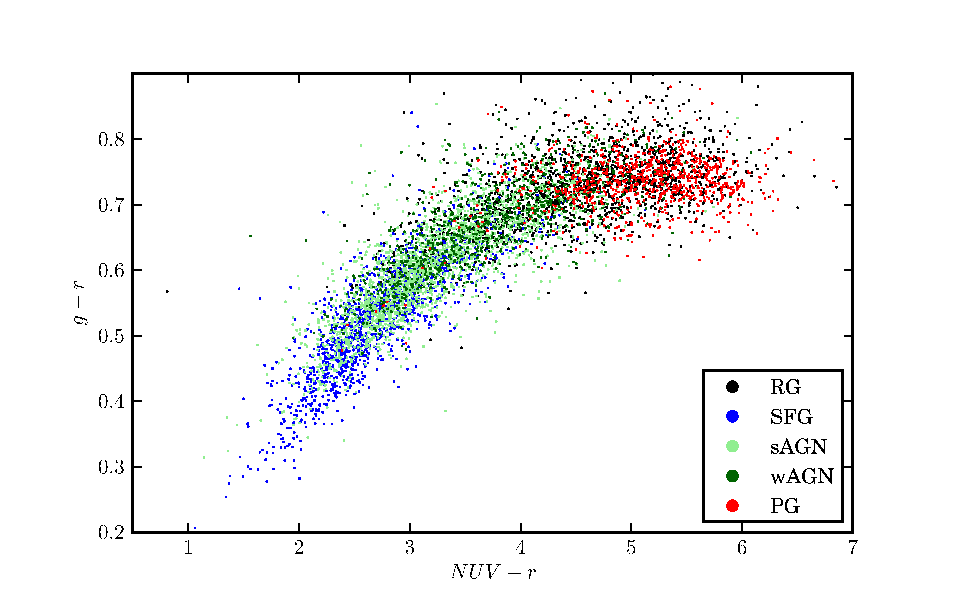
\includegraphics{figuras/uvcolor-color-class.eps}
	\caption[Diagrama cor--cor UV de acordo com o tipo de galáxia.]
	{Classes de galáxias no diagrama cor--cor UV. As cores referentes às classes de
	galáxia são as mesmas do diagrama WHAN (figura \ref{fig:Whan}). É possível
	notar uma separação entre as classes, embora não tão clara quanto no diagrama
	WHAN.}
	\label{fig:ColorClass}
\end{figure}

\begin{figure}
	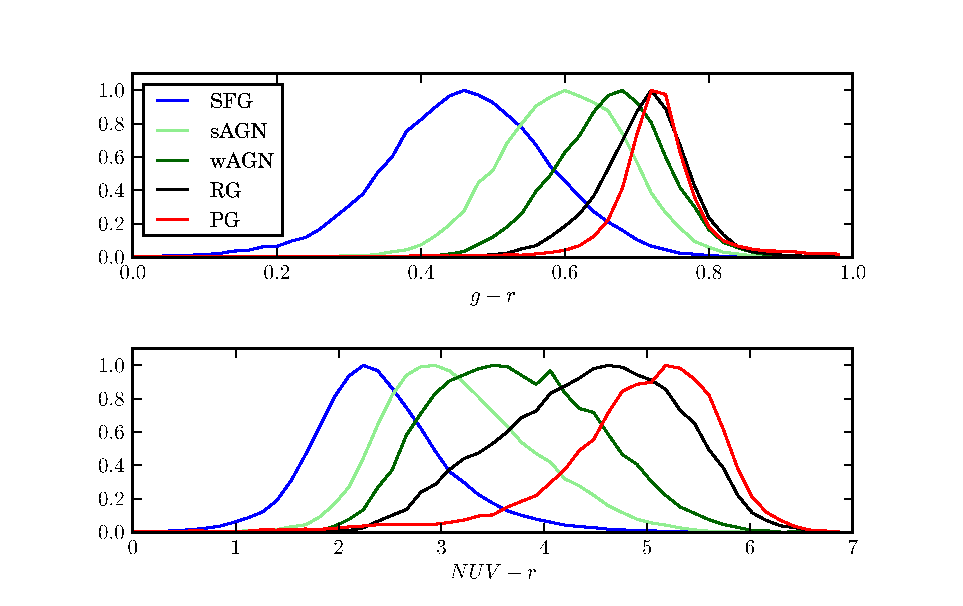
\includegraphics{figuras/histo_galtype_color.eps}
	\caption[Histogramas de cores para as classes de galáxias.]
	{Histogramas normalizado das cores óptica ($g-r$) e ultravioleta ($NUV-r$) para
	as classes de galáxias. A cor das linhas representa a classe conforme a figura
	\ref{fig:Whan}. Em ultravioleta a separação entre as classes de galáxias
	aposentadas (RG) e passivas (PG) torna-se mais clara. Note que os histogramas
	seguem o agrupamento das classes na figura \ref{fig:ColorClass}.}
	\label{fig:HistogramaCorClasse}
\end{figure}


\section{Análise das propriedades físicas}

% TODO: Parâmetros físicos das galáxias no diagrama de cores.
TODO: Parâmetros físicos das galáxias no diagrama de cores.


\begin{figure}
	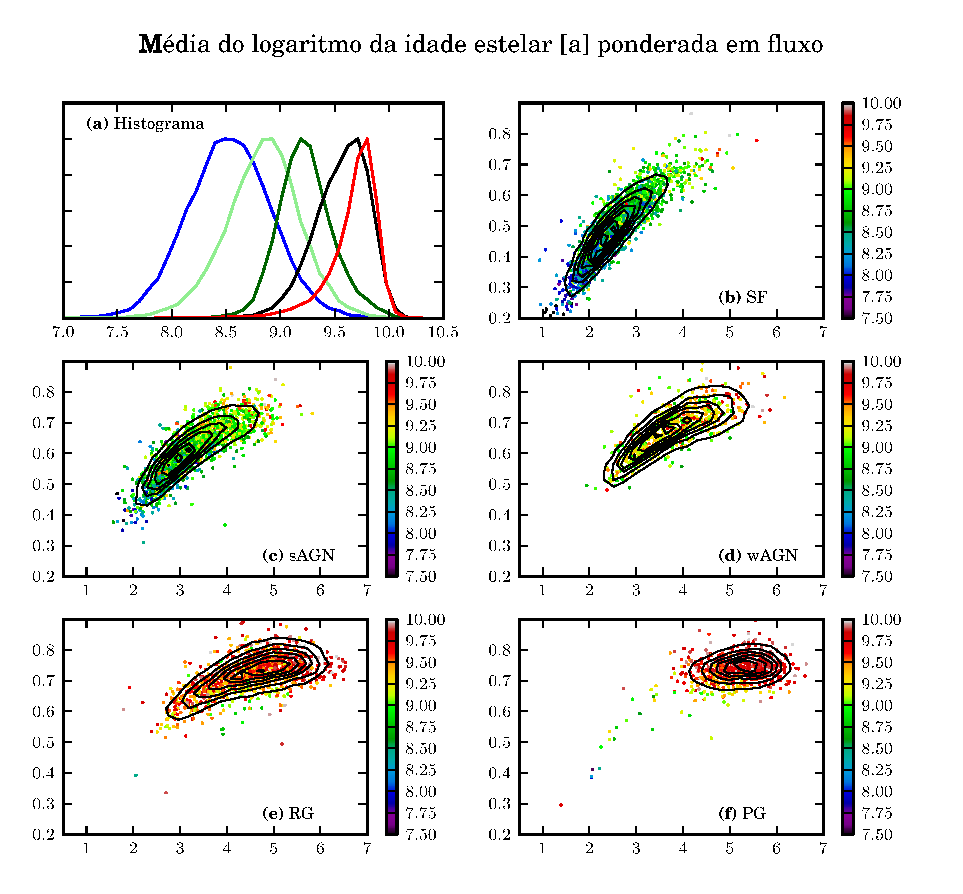
\includegraphics{figuras/uvcolor-color-at_flux-byclass.eps}
	\caption[Idade média das galáxias ponderada em fluxo no diagrama cor--cor UV.]
	{Idade média das galáxias ponderada em fluxo em função de $NUV-r$ e $g-r$. O
	painel \textbf{(a)} contém todas as galáxias da amostra. Os painéis de
	\textbf{(b)} a \textbf{(f)} contém apenas as galáxias con formação estelar
	(SFG), AGN fortes (sAGN), AGN fracas (wAGN), galáxias aposentadas (RG) e
	galáxias passivas (PG), respectivamente. Os contornos indicam a densidade de
	galáxias. A idade média da distribuição vai aumentando conforme a classe, na
	sequência apresentada.}
	\label{fig:ATFluxColor}
\end{figure}

\begin{figure}
	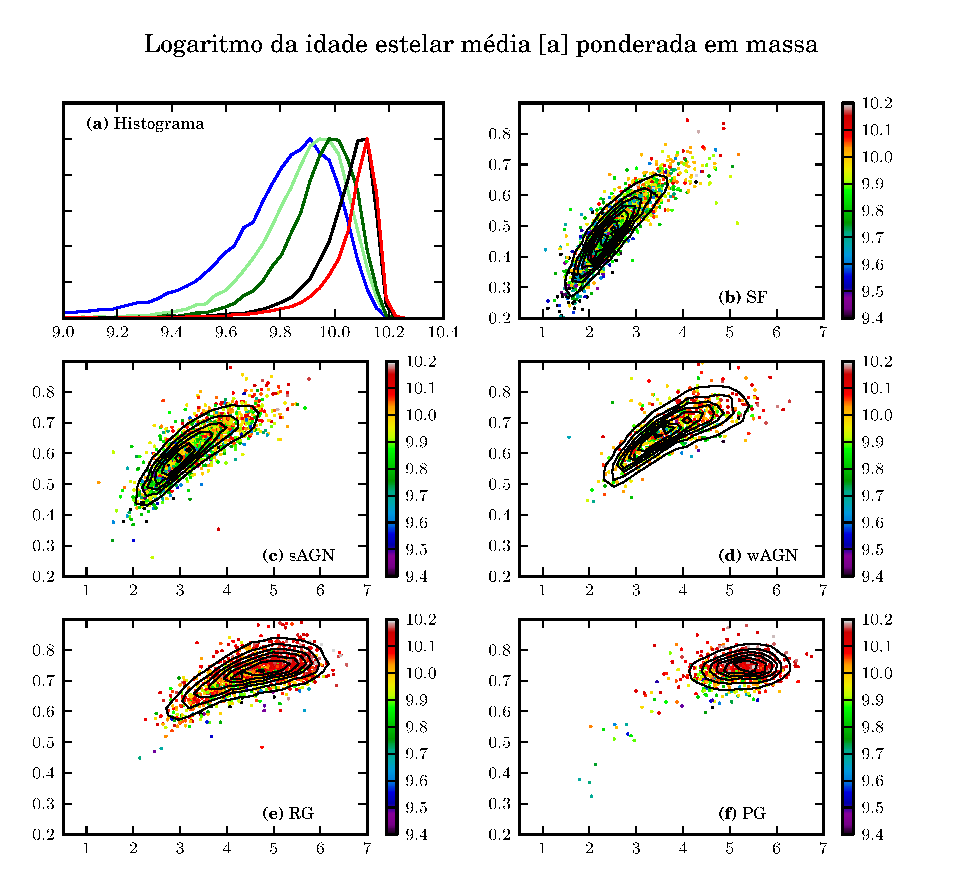
\includegraphics{figuras/uvcolor-color-at_mass-byclass.eps}
	\caption[Idade média das galáxias ponderada em massa no diagrama cor--cor UV.]
	{O mesmo que a figura \ref{fig:ATFluxColor}, para a idade média das galáxias
	ponderada pela massa das SSP componentes. Note que a escala de idades não é a
	mesma.}
	\label{fig:ATMassColor}
\end{figure}

\begin{figure}
	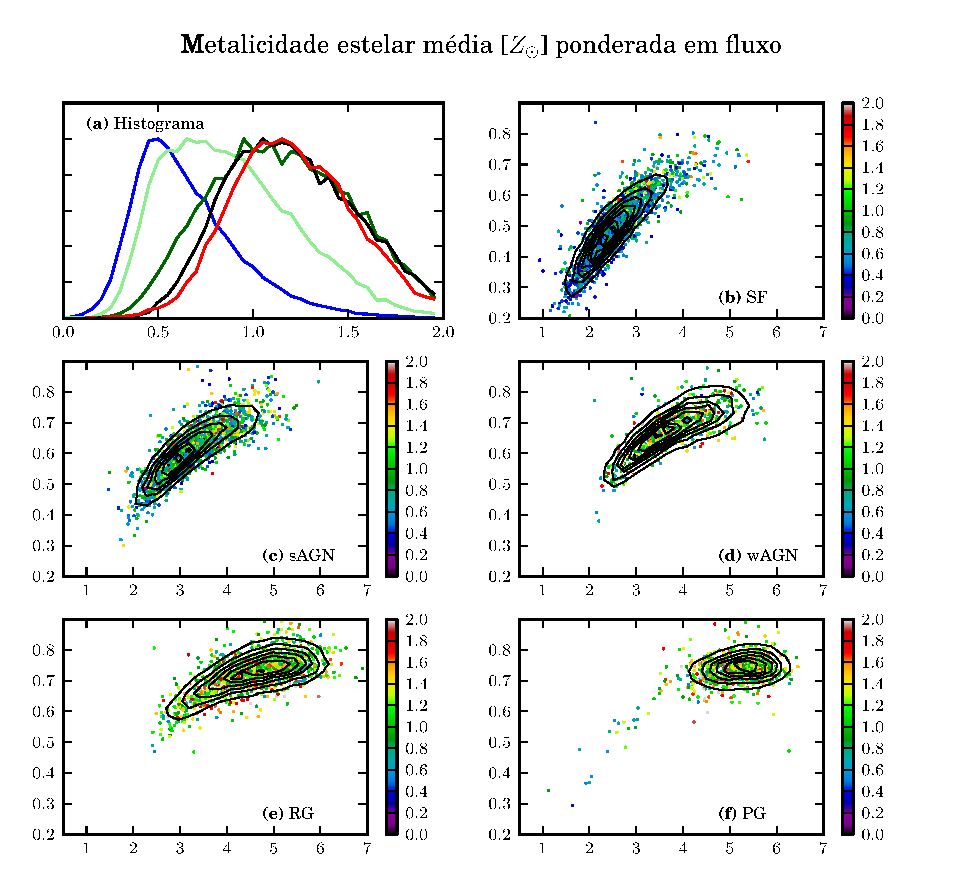
\includegraphics{figuras/uvcolor-color-am_flux-byclass.eps}
	\caption[Metalicidade das galáxias ponderada em fluxo no diagrama cor--cor UV.]
	{O mesmo que a figura \ref{fig:ATFluxColor}, para a metalicidade média das
	galáxias ponderada pelo fluxo das SSP componentes.}
	\label{fig:AMFluxColor}
\end{figure}

\begin{figure}
	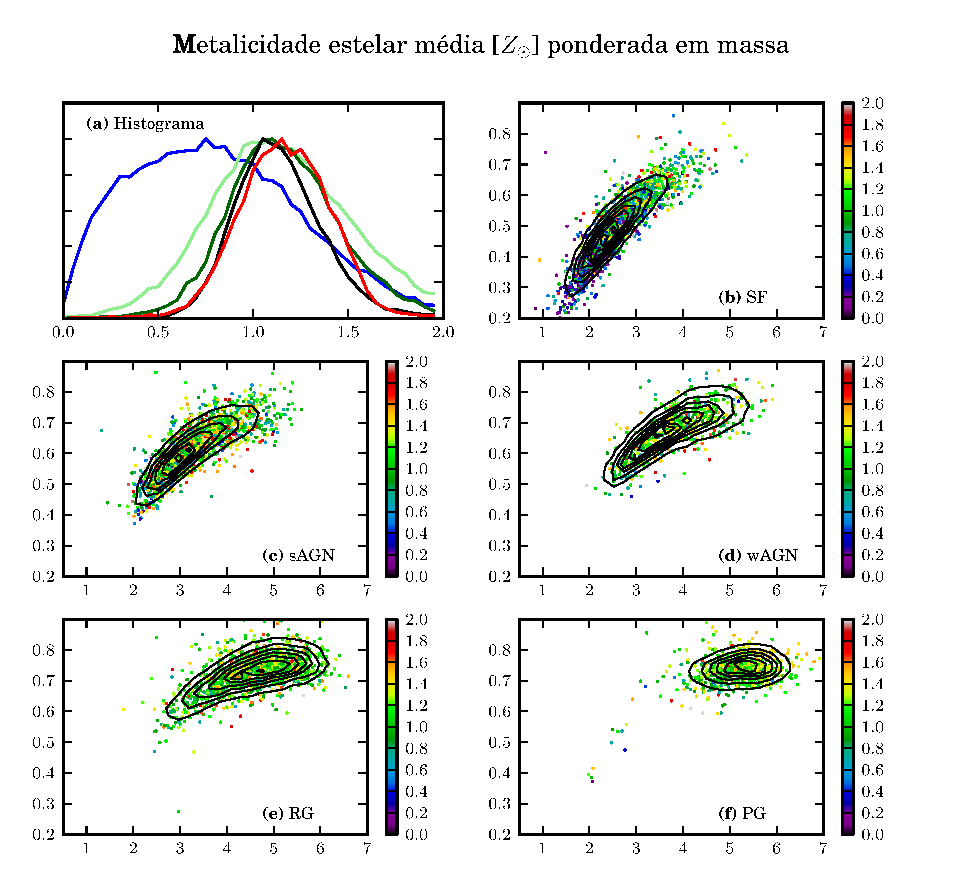
\includegraphics{figuras/uvcolor-color-am_mass-byclass.eps}
	\caption[Metalicidade das galáxias ponderada em massa no diagrama cor--cor UV.]
	{O mesmo que a figura \ref{fig:ATFluxColor}, para a metalicidade média das
	galáxias ponderada pelo massa das SSP componentes.}
	\label{fig:AMMassColor}
\end{figure}

\begin{figure}
	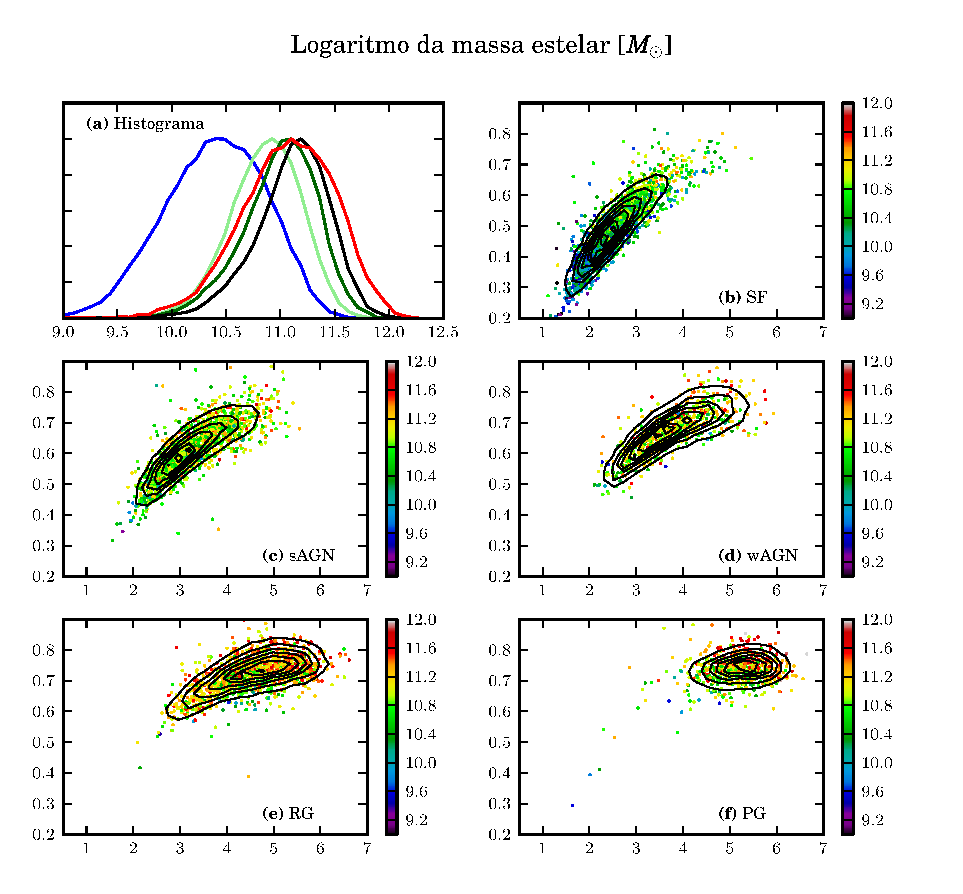
\includegraphics{figuras/uvcolor-color-mcor_gal-byclass.eps}
	\caption[Massa estelar das galáxias no diagrama cor--cor UV.]
	{O mesmo que a figura \ref{fig:ATFluxColor}, para o logaritmo da massa estelar
	das galáxias em massas solares.}
	\label{fig:MCorGalColor}
\end{figure}

\begin{figure}
	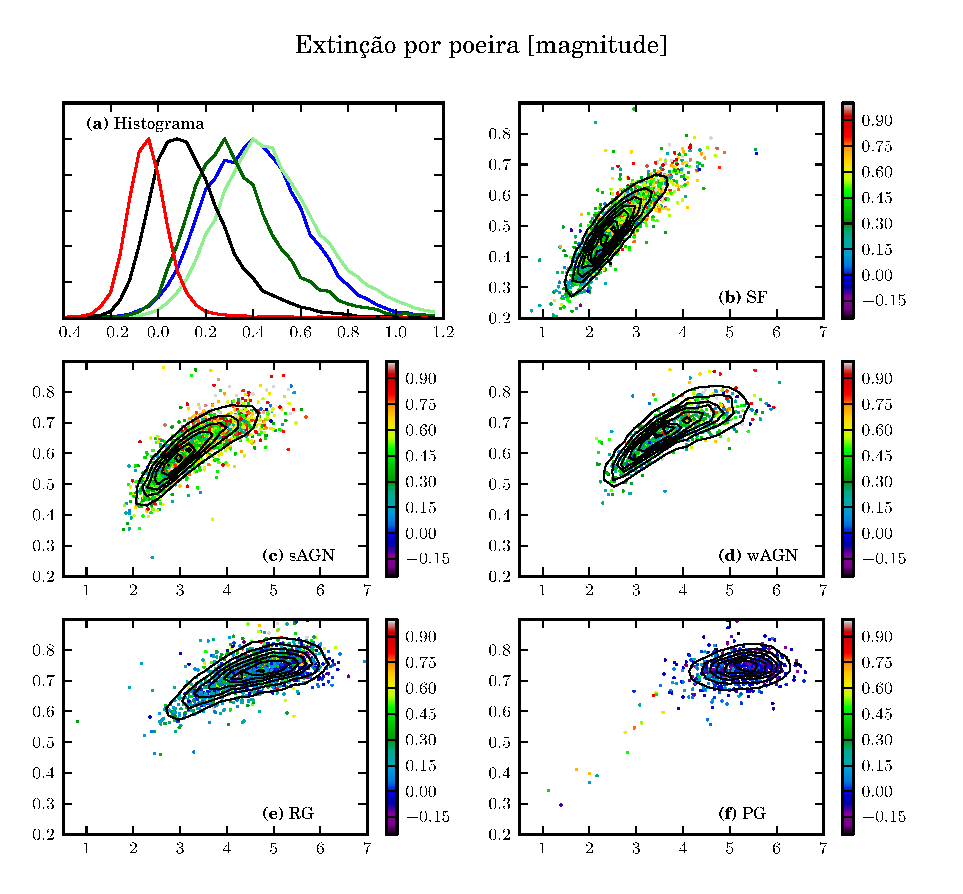
\includegraphics{figuras/uvcolor-color-AV-byclass.eps}
	\caption[Absorção por poeira no diagrama cor--cor UV.]
	{O mesmo que a figura \ref{fig:ATFluxColor}, para a extinção por
	poeira na banda V das galáxias.}
	\label{fig:AVColor}
\end{figure}

\begin{figure}
	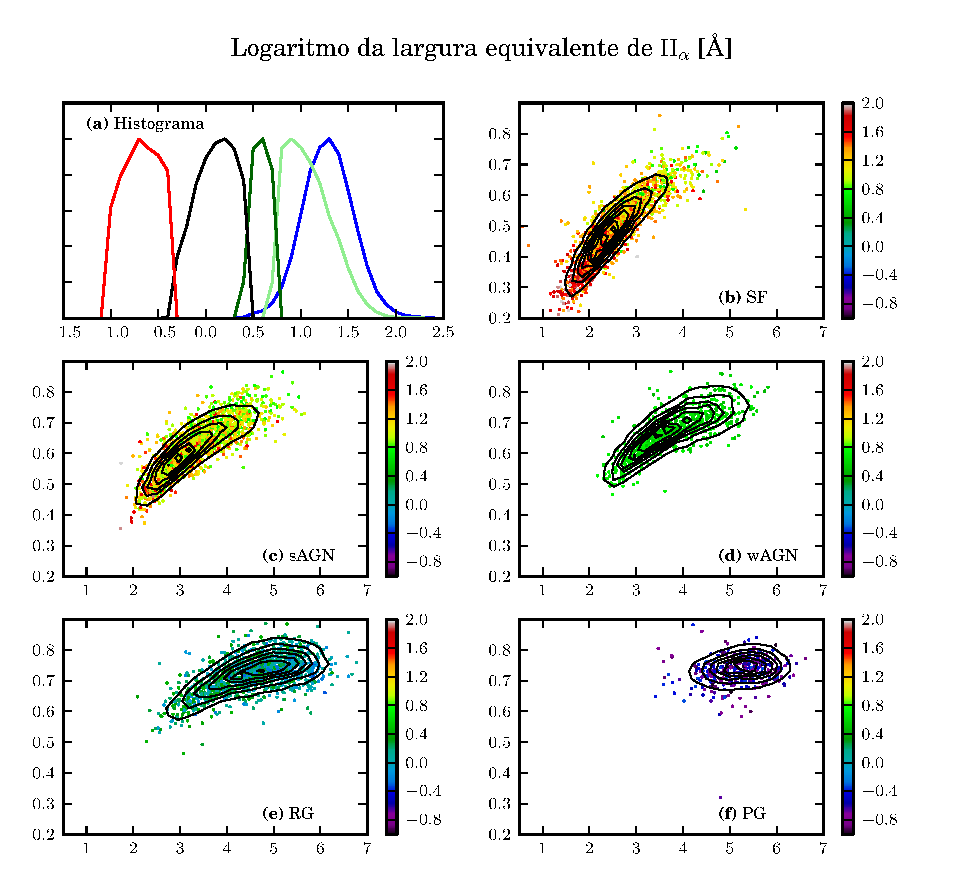
\includegraphics{figuras/uvcolor-color-halpha_ew-byclass.eps}
	\caption[Largura equivalente de \Halpha no diagrama cor--cor UV.]
	{O mesmo que a figura \ref{fig:ATFluxColor}, para o logaritmo da largura
	equivalente de \Halpha das galáxias.}
	\label{fig:EWHaColor}
\end{figure}

\section{Discussão}

\subsection{A separação entre galáxias aposentadas e passivas}

%TODO: Comparar galáxias aposentadas com passivas
TODO: Comparar galáxias aposentadas com passivas
\citep[In prep. perpetuum]{Mateus2013}.


% End of this chapter
